\begin{frame}[plain]
  \begin{tikzpicture}[remember picture,overlay,x=0.1666667mm,y=-0.1666667mm]
    \begin{scope}[shift={(current page.north west)}]

      \slideheader{EDA: геометрия пространства эмбеддингов}

      \node[anchor=north west, inner sep=0pt] at (48,112) {%
        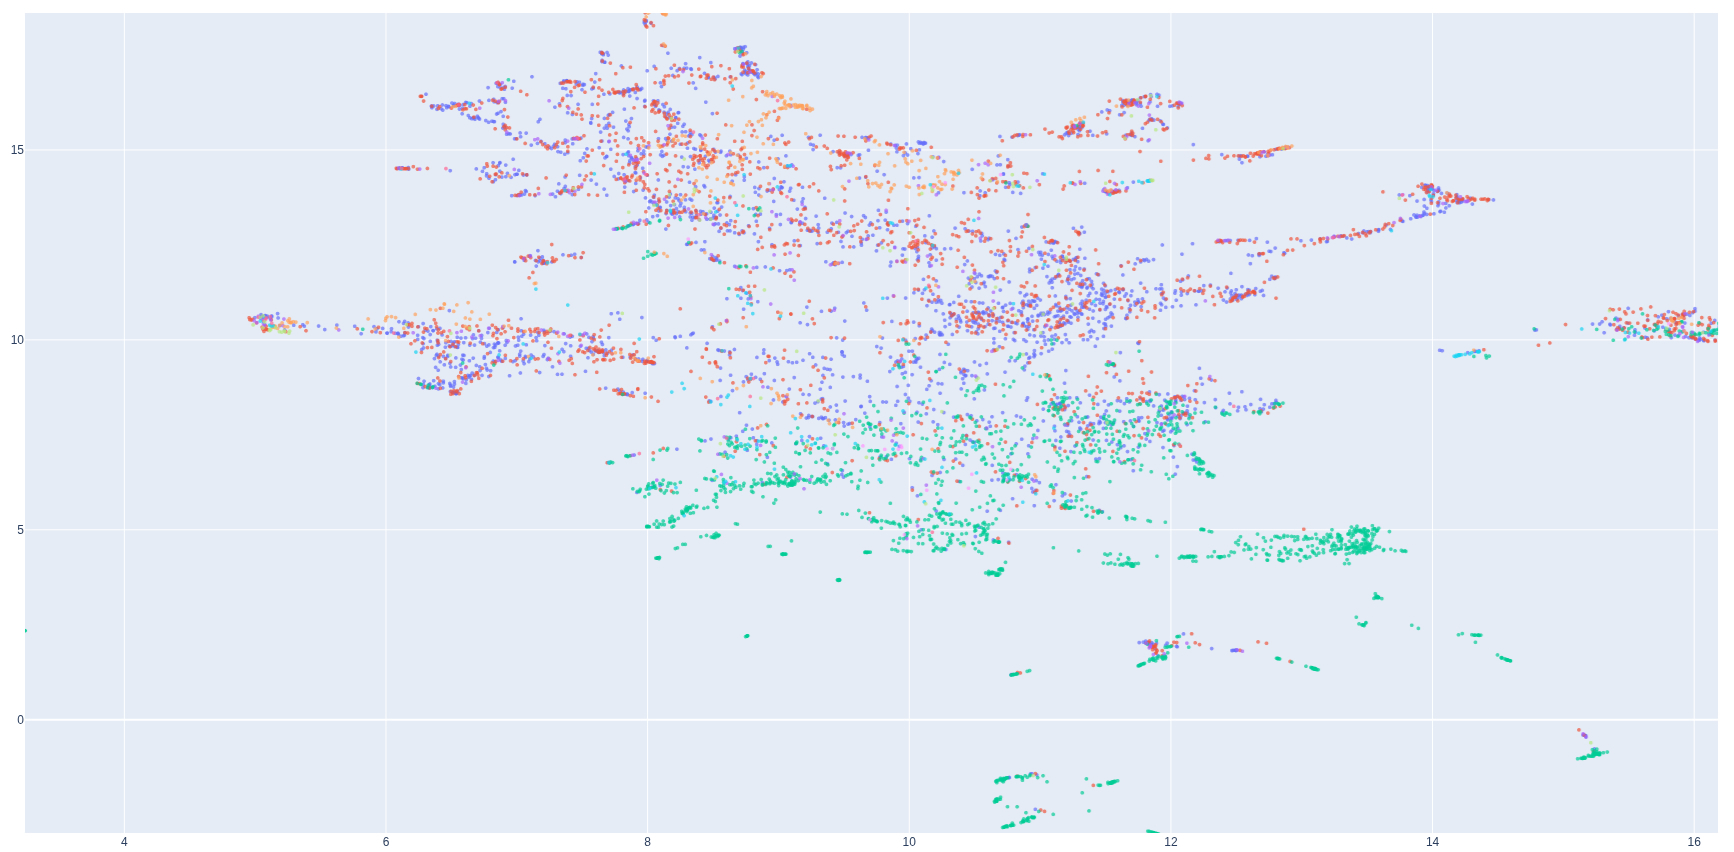
\includegraphics[width=68mm,height=24.2mm]{images/08_calm_by_channel.jpg}%
      };
      \node[anchor=north west, inner sep=0pt] at (504,112) {%
        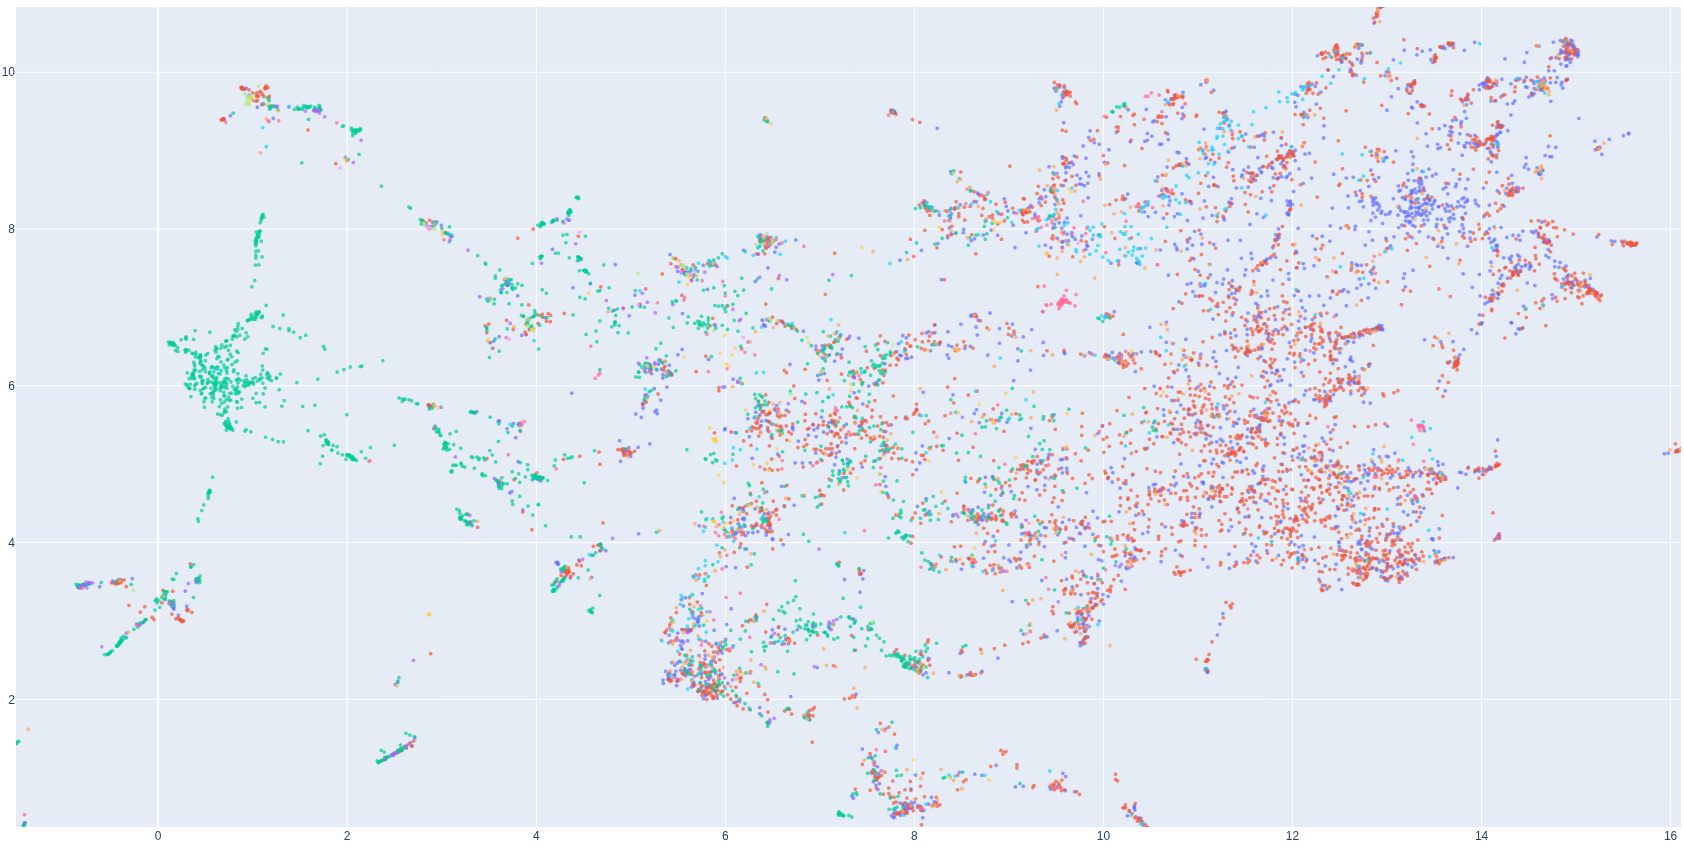
\includegraphics[width=68mm,height=24.2mm]{images/08_war_by_channel.jpg}%
      };
      \node[anchor=north west, inner sep=0pt] at (48,295) {%
        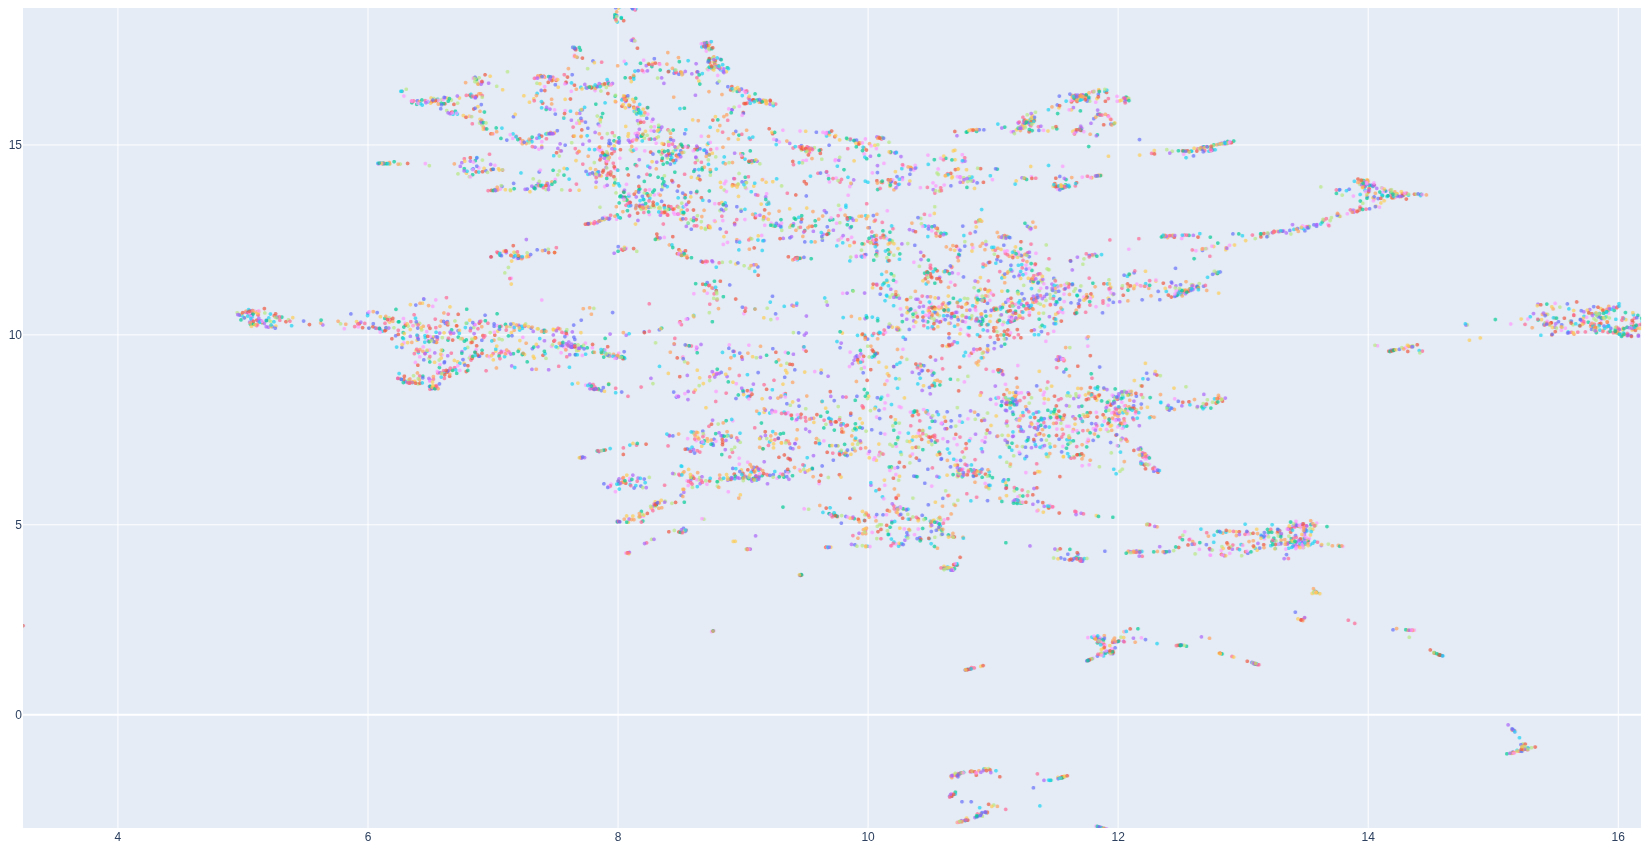
\includegraphics[width=68mm,height=24.2mm]{images/08_calm_by_date.jpg}%
      };
      \node[anchor=north west, inner sep=0pt] at (504,295) {%
        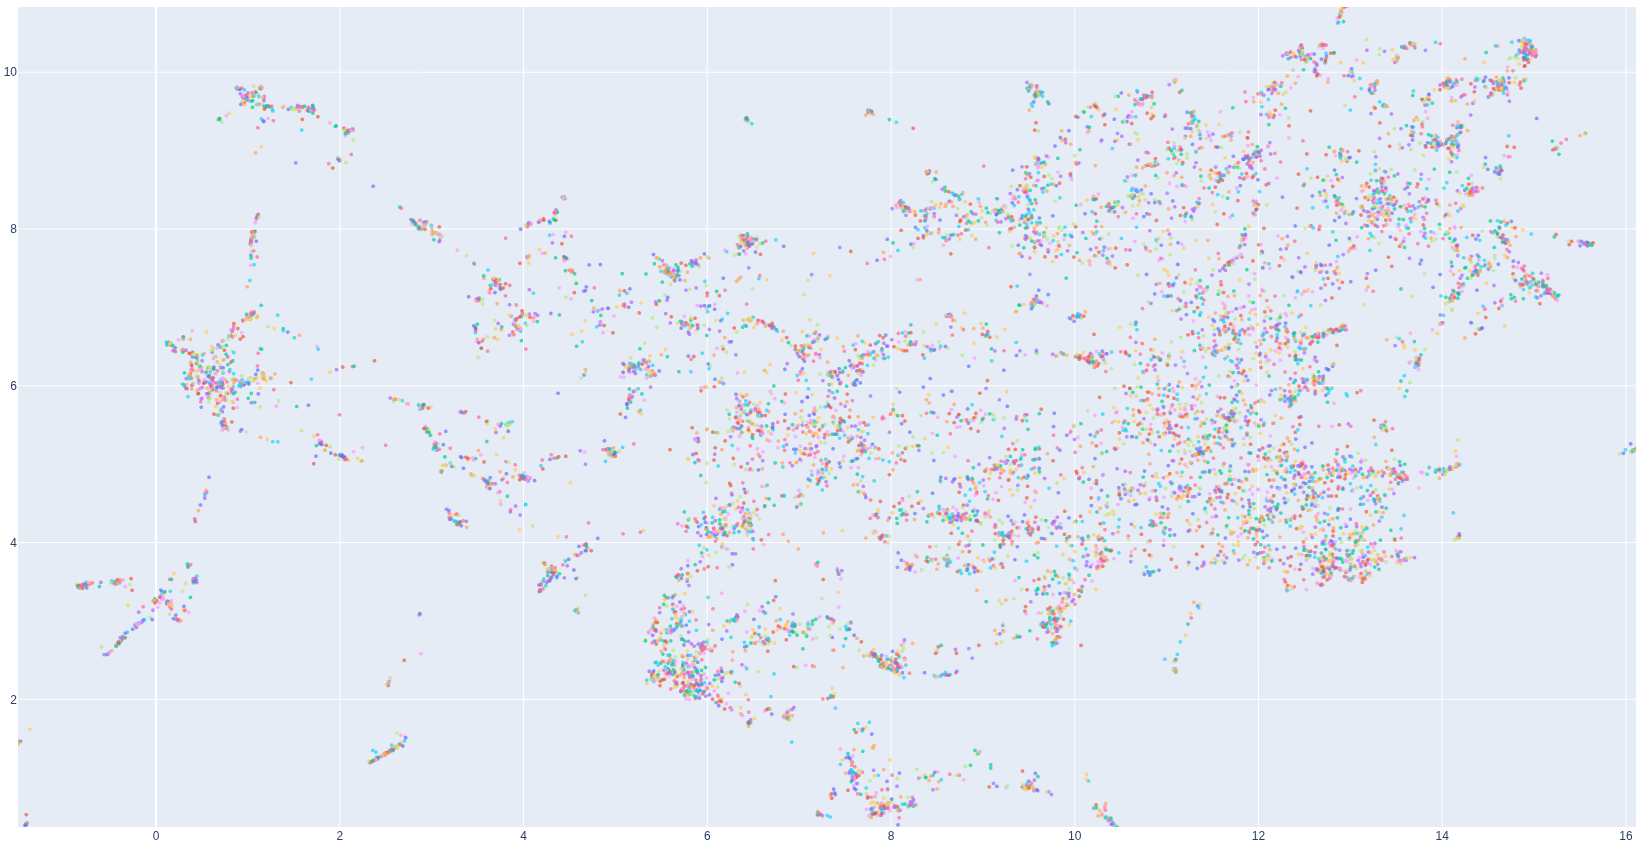
\includegraphics[width=68mm,height=24.2mm]{images/08_war_by_date.jpg}%
      };

      \node[anchor=north, inner sep=0pt, text=BPMuted, font=\scriptsize]
        at (252,268) {спокойный период · по каналам};
      \node[anchor=north, inner sep=0pt, text=BPMuted, font=\scriptsize]
        at (708,268) {санкционный шок · по каналам};
      \node[anchor=north, inner sep=0pt, text=BPMuted, font=\scriptsize]
        at (252,451) {спокойный период · по дате};
      \node[anchor=north, inner sep=0pt, text=BPMuted, font=\scriptsize]
        at (708,451) {санкционный шок · по дате};

      \node[anchor=east, inner sep=0pt, text=BPMuted, font=\scriptsize]
        (primeone) at (546,190) {\texttt{prime1}};
      \draw[-{Latex[length=1.8mm,width=1.2mm]}, draw=BPMuted, line width=0.35mm]
        (primeone.east) -- (565,163);

      \node[anchor=north west, inner sep=0pt, text=BPMuted, font=\scriptsize]
        at (64,472) {• каналы перемешаны в основном облаке — source bias отсутствует};
      \node[anchor=north west, inner sep=0pt, text=BPMuted, font=\scriptsize]
        at (64,490) {• цвета по дате равномерны внутри окна — temporal drift отсутствует};

      \slidefooter{Сергей Устьянцев}{Извлечение сигнала инфляционных ожиданий
из новостного потока с контролем утечки будущих данных}

    \end{scope}
  \end{tikzpicture}
\end{frame}
